
\documentclass[a4paper]{article}
\usepackage[english]{babel}
\usepackage[utf8]{inputenc}
\usepackage{amsmath}
\usepackage{graphicx}
\usepackage{float}
\usepackage{hyperref}
\usepackage{multicol}
\usepackage{comment}
\usepackage{mathtools}
\usepackage[margin=0.7in]{geometry}

\usepackage{xcolor}
\setlength{\parindent}{0 pt}
\setlength{\parskip}{1em} 
\usepackage{physics}


\usepackage{xcolor}
\usepackage[most]{tcolorbox}
\usepackage{listings}

\usepackage{xparse}

\NewDocumentCommand{\codeword}{v}{%
\texttt{\textcolor{blue}{#1}}%
}


\definecolor{white}{rgb}{1,1,1}
\definecolor{mygreen}{rgb}{0,0.4,0}
\definecolor{light_gray}{rgb}{0.97,0.97,0.97}
\definecolor{mykey}{rgb}{0.117,0.403,0.713}

\tcbuselibrary{listings}
\newlength\inwd
\setlength\inwd{1.3cm}

\newcounter{ipythcntr}
\renewcommand{\theipythcntr}{\texttt{[\arabic{ipythcntr}]}}

\newtcblisting{pyin}[1][]{%
  sharp corners,
  enlarge left by=\inwd,
  width=\linewidth- 1.2\inwd,
  enhanced,
  boxrule=0pt,
  colback=light_gray,
  listing only,
  top=0pt,
  bottom=0pt,
  overlay={
    \node[
      anchor=north east,
      text width=\inwd,
      font=\footnotesize\ttfamily\color{mykey},
      inner ysep=2mm,
      inner xsep=0pt,
      outer sep=0pt
      ] 
      at (frame.north west)
      {\refstepcounter{ipythcntr}\label{#1}In \theipythcntr:};
  }
  listing engine=listing,
  listing options={
    aboveskip=1pt,
    belowskip=1pt,
    basicstyle=\footnotesize\ttfamily,
    language=Python,
    keywordstyle=\color{mykey},
    showstringspaces=false,
    stringstyle=\color{mygreen},
    commentstyle=\color{mygreen}
  },
}
\newtcblisting{pyprint}{
  sharp corners,
  enlarge left by=\inwd,
  width=\linewidth-1.2\inwd,
  enhanced,
  boxrule=0pt,
  colback=white,
  listing only,
  top=0pt,
  bottom=0pt,
  overlay={
    \node[
      anchor=north east,
      text width=\inwd,
      font=\footnotesize\ttfamily\color{mykey},
      inner ysep=2mm,
      inner xsep=0pt,
      outer sep=0pt
      ] 
      at (frame.north west)
      {};
  }
  listing engine=listing,
  listing options={
      aboveskip=1pt,
      belowskip=1pt,
      basicstyle=\footnotesize\ttfamily,
      language=Python,
      keywordstyle=\color{mykey},
      showstringspaces=false,
      stringstyle=\color{mygreen}
    },
}
\newtcblisting{pyout}[1][\theipythcntr]{
  sharp corners,
  enlarge left by=\inwd,
  width=\linewidth-\inwd,
  enhanced,
  boxrule=0pt,
  colback=white,
  listing only,
  top=0pt,
  bottom=0pt,
  overlay={
    \node[
      anchor=north east,
      text width=\inwd,
      font=\footnotesize\ttfamily\color{mykey},
      inner ysep=2mm,
      inner xsep=0pt,
      outer sep=0pt
      ] 
      at (frame.north west)
      {\setcounter{ipythcntr}{\value{ipythcntr}}Out#1:};
  }
  listing engine=listing,
  listing options={
      aboveskip=1pt,
      belowskip=1pt,
      basicstyle=\footnotesize\ttfamily,
      language=Python,
      keywordstyle=\color{mykey},
      showstringspaces=false,
      stringstyle=\color{mygreen}
    },
}


\newsavebox{\selvestebox}
\newenvironment{colbox}[1]
  {\newcommand\colboxcolor{#1}%
   \begin{lrbox}{\selvestebox}%
   \begin{minipage}{\dimexpr\columnwidth-2\fboxsep\relax}}
  {\end{minipage}\end{lrbox}%
   \begin{center}
   \colorbox[HTML]{\colboxcolor}{\usebox{\selvestebox}}
   \end{center}}


\title{The Fast Fourier transform \\
\large How to use it, and common pitfalls}
\author{Jo\"elle Begin, July 2020}
\bf
\date{}

\begin{document}
\maketitle

Working in cosmology, you'll be using the Fourier transform \textit{a lot}. Here is the functional form of the Fourier transform, 

\begin{equation*}
    \tilde{f}(k) = \int _{-\infty}^{\infty} dx \  e^{-ikx} f(x)
\end{equation*}

But although the things we study are in reality continuous, when we're dealing with real experimental data or numerical simulations we work with discrete \textbf{samples} of the continuous thing. So, you have to be able to do a numerical Fourier transform for all your discrete data!

Luckily, you don't have to re-invent the wheel. Some clever programmers already came up with an algorithm for computing the discrete Fourier transform, which numpy has helpfully wrapped in the function \codeword{fft}. Let's see the FFT in practice with a simple example. Let 

\begin{equation*}
    f(x) = \sin(\frac{2\pi x}{L})
\end{equation*}

Then the Fourier transform will be 

\begin{equation*}
    \tilde{f}(k) = \frac{1}{2i}\qty[\delta \qty(k + \frac{2\pi}{L}) - \delta \qty(k - \frac{2\pi}{L})]
\end{equation*}

So we should expect a completely imaginary signal, with spikes at $k = 2\pi/L$ and $k = -2\pi/L$. Let's see what the code does!


\begin{pyin}
import numpy as np
import matplotlib.pyplot as plt 
from numpy.fft import fft
    
def function(x, L):
    return np.sin(2*np.pi*x/L)

L = np.pi
x = np.linspace(-2*np.pi,2*np.pi,200)

f = function(x, L)
f_tilde = fft(f)
\end{pyin}
    
So we have a pure sine wave as our function 

\begin{figure}[H]
    \centering
    \includegraphics[width = 0.5\linewidth]{figures/sin.pdf}
\end{figure}

and when we plot \lstinline{f_tilde}, we get the following:

\begin{figure}[H]
    \centering
    \includegraphics[width = 0.8\linewidth]{figures/first_fft.pdf}
\end{figure}

Uh-oh. Something strange is going on. The first thing that seems weird is that the real part is not zero, as we would have expected. What's happening here?

\begin{colbox}{F8E0E0}
    \textbf{FFT PITFALL}: The FFT algorithm assumes periodic boundary conditions.
\end{colbox}

We're giving the FFT what we think is a pure sine wave, but the FFT effectively tiles this signal we're giving it. It assumes your input is a sample of exactly one period of an infinite periodic signal. So, after tiling, is it a pure sine wave? Let's try the following:
\begin{pyin}
x_tiled = np.linspace(0,8*np.pi,400)
tiled = [list(f)*2][0]
\end{pyin} 

\vspace{2pt}

and plot what the tiled function looks like. 

\begin{figure}[H]
    \centering
    \includegraphics[width = 0.9\linewidth]{figures/tiling.pdf}
\end{figure}

Aha! There's a little hump right where we tile the two sine waves. This is because if you look at how we defined our range of angles above, we did \codeword{np.linspace(-2*np.pi,2*np.pi,200)}. This means that \codeword{f[0] = 0} and \codeword{f[-1] = 0}, so when the FFT algorithm applies periodic boundary conditions, there will be two zeros in series. That is, in FFT's eyes, this is not a pure sine wave! Let's give FFT a pure sine wave now.

\begin{pyin}
pure_sine = f[:-1] #popping out last element that would give repeated zeros
pure_sine_tilde = fft(pure_sine)
\end{pyin}

Now, plotting \codeword{pure_sine_tilde}:

\begin{figure}[H]
    \centering
    \includegraphics[width = 0.8\linewidth]{figures/fourier_2.pdf}
\end{figure}

Exactly as we expected! Wonderful! We've dodged the first FFT pitfall. But let's keep going, cause trust me, there are many more. How about the location of the peaks? We expect spikes at $k = 2\pi /L$ and $k = -2\pi / L$. Note that I haven't told \codeword{matplotlib} what goes on the x-axis yet, so let's see how FFT decides where to put the peaks. Let's look at this picture from the fantastic book \textit{Numerical Recipes}.

\begin{figure}[H]
    \centering
    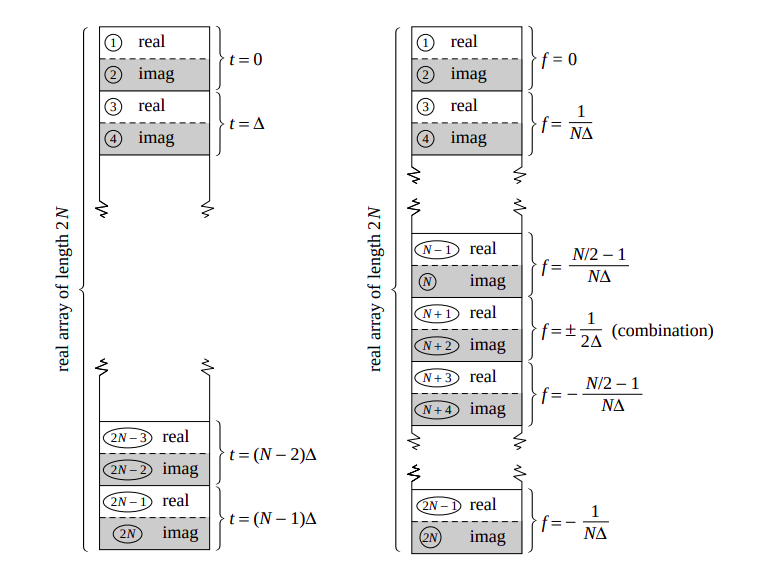
\includegraphics[width = 0.8\linewidth]{figures/fft.png}
    \caption{FFT diagram from \textit{Numerical Recipes}}
    \label{fig:fft}
\end{figure}

There's a lot to unpack here. The panel on the left is a representation of the input that FFT expects. The algorithm assumes an input of $N$ elements\footnote{Here they have $2N$ elements because in the programming language this textbook is written there is no complex data type, so they represent a complex array of some signal $S$ by letting \lstinline{array[i] =} Re($S_i$) and \lstinline{array[i+1] =} Im($S_i$).}, sampled at a resolution of $\Delta$. Then, after the FFT has been computed, the output in Fourier space has a resolution of 

\begin{equation*}
    \Delta f = \frac{1}{N\Delta}
\end{equation*}

Which is known as the \textit{nyquist frequency}. So the values returned by \codeword{fft} correspond to the Fourier transform sampled at $1/ N \Delta$, $2/ N\Delta$, and so on. Again, numpy has a nice function that takes care of this for us. 

\begin{pyin}
from numpy.fft import fftfreq

Delta = x[1] - x[0]
freqs = fftfreq(len(pure_sine), Delta)

nyquist_theory = 1/(len(pure_sine)*Delta)
nyquist_fft = freqs[1]

print("Theoretical nyquist frequency: ", nyquist_theory)
print("fftfreqs nyquist frequency: ", nyquist_fft)
\end{pyin}
\vspace{1px}
\begin{pyprint}
Theoretical nyquist frequency:  0.07957747154594787
fftfreqs nyquist frequency:  0.07957747154594787
\end{pyprint}
Now, let's plot our FFT with the proper axis. But first... 


\begin{colbox}{F8E0E0}
    \textbf{FFT PITFALL}: Origin placement. The FFT algorithm has a weird idea of how the data is ordered. 
\end{colbox}

The astute reader will notice from figure~\ref{fig:fft} that the ordering of the frequencies is strange. It goes from the zero frequency, to the largest \textit{positive} frequency, to the \textit{smallest} negative frequency, then finally to the \textit{largest} negative frequency. If you're a normal person and like to order your data like $-\infty \rightarrow 0 \rightarrow \infty$, you have to account for this. As always, numpy to the recue! 
\vspace{1px}
\begin{pyin}
    from numpy.fft import fftshift 

'''technically I should shift the input as well, but in this case 
we don't have to because of periodicity'''
pure_sine_tilde_shifted = fftshift(fft(pure_sine))
freqs_shifted = fftshift(freqs)
\end{pyin}

\begin{figure}[H]
    \centering
    \includegraphics[width = 0.5\linewidth]{figures/shifted.pdf}
\end{figure}

ALright! Looking good. Now, let's locate the peaks.
\\
\begin{pyin}
peak_ind = np.where(pure_sine_tilde_shifted == np.max(pure_sine_tilde_shifted))[0][0]
theoretical_peak = 2*np.pi/L

print("Theoretical peak: ", theoretical_peak)
print("fft peak: ",np.abs(freqs_shifted[peak_ind]))

\end{pyin}

\begin{pyprint}
Theoretical peak:  2.0
fft peak:  0.31830988618379147

\end{pyprint} 

Looks like we have more to do. You guessed it, here comes another... 


\begin{colbox}{F8E0E0}
    \textbf{FFT PITFALL}: Why can't everyone just use the same conventions?
\end{colbox}

The reason that we aren't getting the correct locations for the peaks is that we haven't scaled the horizontal axis properly. The reason we have to scale this axis is because the Fourier convention that we use in cosmology is different than the FFT convention. Here is the FFT convention, from numpy documentation:

\begin{align*}
    A_j = \sum_{m=0}^{N-1} a_m \ \exp[-i2\pi \frac{mj}{N}] \tag{$\star$}
\end{align*}

Now let's take the cosmology convention, and try to get it in a similar form. 

\begin{align*}
    \tilde{f}(k) &= \int dx \ e^{-ikx} f(x) \\
    &\approx \sum_{m=0}^{N-1} (\Delta x) e^{-ikx_m}f(x_m) \\
    &= \sum_{m=0}^{N-1} (\Delta x) f(\Delta m) e^{-ikm\Delta} \tag{$\star \star$}
\end{align*} 

Here we've used 

\begin{equation*}
    x_m = \Delta m
\end{equation*}

since the $m$th sample of the smooth function will correspond to the sampling resolution $\Delta$ times the index $m$. We can set $(\star) = (\star \star)$, and comparing the exponents:

\begin{equation*}
    k_j m \Delta = \frac{2\pi m j}{N}
\end{equation*}

and so 

\begin{equation*}
    k_j = 2\pi \frac{j}{N\Delta}
\end{equation*}

notice that $j / N \Delta$ is exactly the expression we would expect for the $j$th Fourier number, but we have an extra factor of $2\pi$ due to the different Fourier conventions. Then, if we account for this:


\begin{pyin}
k_array = freqs_shifted*2*np.pi
peak_scaled = k_array[peak_ind]

print("Theoretical peak: ", theoretical_peak)
print("fft peak with scaled axis: ",np.abs(peak_scaled))
\end{pyin}

\begin{pyprint}
Theoretical peak:  2.0
fft peak with scaled axis:  2.000000000000005
\end{pyprint}

And we're done! Exactly as we expected! Actually, one last comment.


\begin{colbox}{F8E0E0}
    \textbf{FFT PITFALL}: On scaling the amplitudes.
\end{colbox}

In this example I didn't bother with the amplitudes since it's delta functions, but in general you have to correct for amplitudes as well. Notice from $(\star)$ that this is a dimensionless expression. When we're doing Fourier transforms of physical things, the integrand has dimensions! Again comparing $(\star)$ and $(\star \star)$, 

\begin{equation*}
    a_m = (\Delta x)f(\Delta m)
\end{equation*}

So if I have my array \codeword{f} corresponding to the discretely sampled function, in order to have a proper normalization I would have to do: 

\begin{pyin}
    f_tilde = fft(fftshift(fft(f*delta_x)))
\end{pyin}

where \codeword{delta_x} is my real space resolution. \textbf{Units matter here!!!}. If I have some volume of length $L$ Mpc, with resolution $\Delta$ Mpc and $N$ samples, then my k-space resolution will be 

\begin{equation*}
    \Delta k = \frac{2\pi}{L} = \frac{2\pi}{N\Delta}
\end{equation*}

so it is very important to be watchful of units here. \\


\textbf{Some closing thoughts}: This was long, but I hope having read this will save you some of the long hours I've spent trying to figure out FFT. You will probably make some mistakes; I've been working with FFT for over a year now, and still learned some new things in writing this. But don't feel bad, it is a \textit{very} counter-intuitive algorthim, riddled with pitfalls. So, best of luck!
\end{document}
